\documentclass[10, sigconf]{acmart}

\usepackage{graphicx,xspace,verbatim,comment}
\usepackage{hyperref,array,color,balance,multirow}
\usepackage{balance,float,url,amsfonts,alltt}
\usepackage{mathtools,rotating,amsmath,amssymb}
\usepackage{color,ifpdf,fancyvrb}
\usepackage{etoolbox,listings,subcaption}
\usepackage{bigstrut,morefloats,pbox}
\usepackage{amsmath}
\usepackage{algorithm}
\usepackage[noend]{algpseudocode}
\usepackage{booktabs}

\newtheorem{theorem}{Theorem}[section]
\newtheorem{proposition}{Proposition}[section]
\newtheorem{corollary}[theorem]{Corollary}
\newtheorem{lemma}[theorem]{Lemma}
\newtheorem{definition}{Definition}[section]
\newcommand{\eat}[1]{}
\newcommand{\red}{\textcolor{red}}
\newcommand{\system}{\textsc{Krypton}}

\makeatletter
\def\BState{\State\hskip-\ALG@thistlm}
\makeatother 

\newenvironment{packeditems}{
\begin{itemize}
  \setlength{\itemsep}{1pt}
  \setlength{\parskip}{0pt}
  \setlength{\parsep}{0pt}
}{\end{itemize}}

\newenvironment{packedenums}{
\begin{enumerate}
  \setlength{\itemsep}{1pt}
  \setlength{\parskip}{0pt}
  \setlength{\parsep}{0pt}
}{\end{enumerate}}


\newcolumntype{P}[1]{>{\centering\arraybackslash}p{#1}}

\DeclareMathOperator*{\argmin}{arg\,min}

\setcopyright{none}
\settopmatter{printacmref=false}
\renewcommand\footnotetextcopyrightpermission[1]{} % removes footnote with 
\pagestyle{plain} % removes running headers

\begin{document}
\title{\textsc{Kryton}: A System for Accelerating Occlusion based Deep CNN Explainability Workloads}

\author{Supun Nakandala \hspace{7mm} Arun Kumar}
\affiliation{%
  \institution{University of California, San Diego}
}
\email{{snakanda, arunkk}@eng.ucsd.edu}


\begin{abstract}
Deep Convolution Neural Networks (CNN) have revolutionized the field of computer vision with even surpassing human level accuracy in some of the image recognition tasks such as ImageNet challenge. Thus they are now being deployed in many real-world use cases using a paradigm called \textit{transfer learning}. However one of the major criticisms pointed against Deep CNNs is the black-box nature of how they make predictions. This is a critical issue when applying CNN based approaches to critical applications such as in health care where the explainability of the predictions is also very important. For interpreting CNN predictions several approaches has been proposed and one of the widely used method in image classification tasks is occlusion experiments. In occlusion experiments one would mask the regions of the input image using a small grey or black patch and record the change in the predicted label probability. By systematically changing the position of the patch location, a sensitivity map can be generated from which the regions in the input image which influence the predicted class label most can be identified. However, this method requires performing multiple forward passes of CNN inference for explaining a single prediction and hence very time consuming.
We present \system, the first data system to elevate occlusion experiments to a declarative level and enable automated \textit{incremental} and \textit{approximate} inference optimizations. Experiments with real-world datasets and deep CNNs show that \system~can enable up to 10x speedups.
\end{abstract}

\maketitle

%!TEX root = <main.tex>
\section{Introduction}
Deep Convolution Neural Networks (CNNs) are now the state of the art method for many image prediction tasks~\cite{imagenet}. Thus, there is growing interest in adopting deep CNNs in various application domains, including healthcare~\cite{kermany2018identifying, islam2017abnormality}, agriculture~\cite{mohanty2016using}, security~\cite{arbabzadah2016identifying}, and sociology~\cite{wang2017deep}. Remarkably, even the US Food and Drug Administration recently approved the use of deep CNNs in radiology to assist radiologists in processing X-rays and other scans, cross-checking their decisions, and even mitigating the shortage of radiologists~\cite{fdaretinopathy,radiologistshortage}.

\begin{figure}[t]
% \vspace{-4mm}
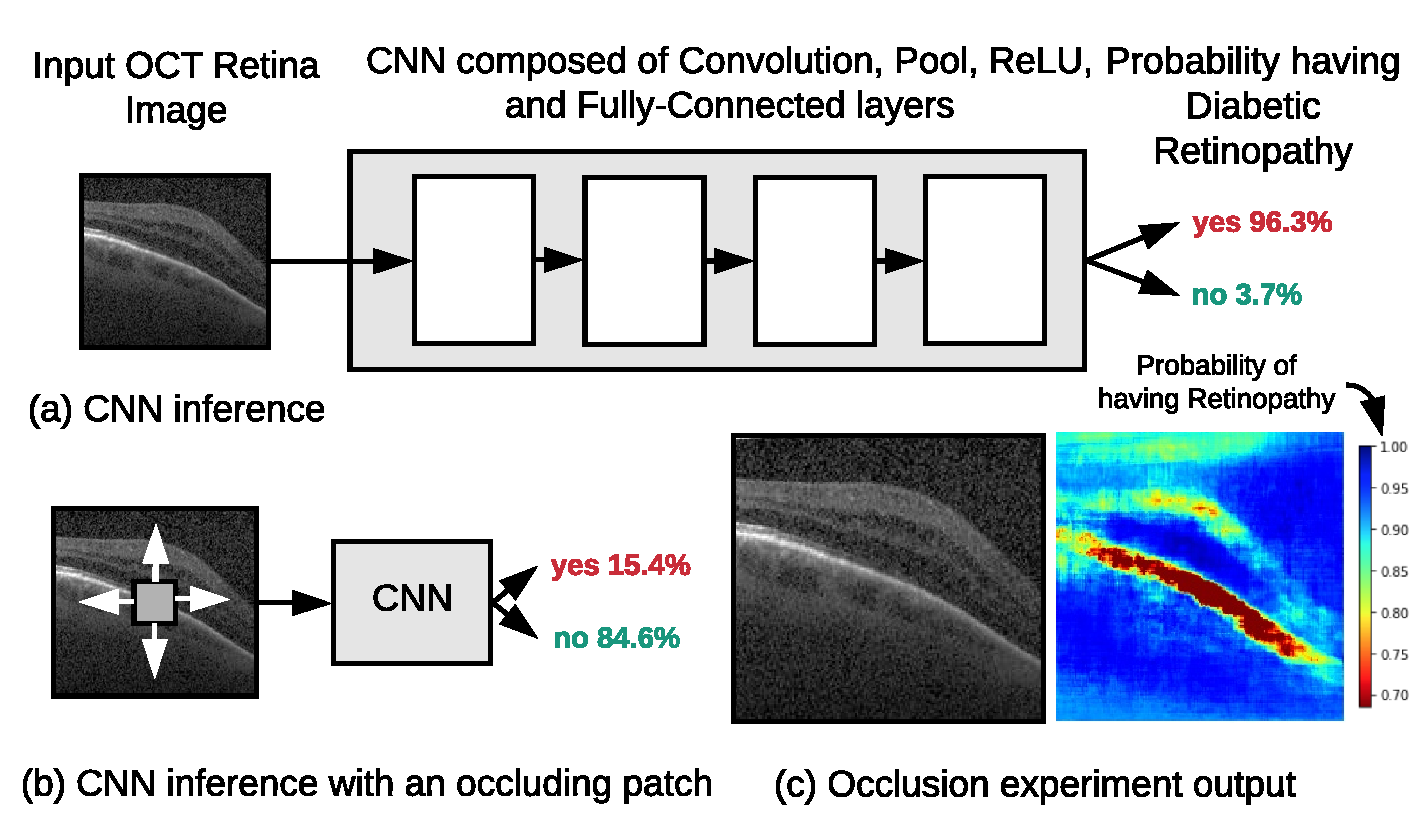
\includegraphics[width=\columnwidth]{./images/krypton_overview}
\caption{(a) Using a CNN to predict diabetic retinopathy in an OCT image/scan. (b) Occluding a part of the image changes the prediction probability. (c) By moving the occluding patch, a sensitivity heat map can be produced.}
\label{fig:krypton_overview}
\vspace{-4mm}
\end{figure}

Despite their successes, a key criticism of CNNs is that their internal workings are unintuitive to non-technical users. Thus, users often seek an ``explanation'' for why a CNN predicted a certain label. Explanations can help users trust CNNs~\cite{ribeiro2016should}, especially in high stakes applications such as radiology~\cite{jung2017deep}, and are a legal requirement for machine learning applications in some countries~\cite{gdpr}. How to explain a CNN prediction is still an active research question, but in the practical literature, an already popular mechanism for CNN explanations is a simple procedure called \textit{occlusion-based explanations}~\cite{zeiler2014visualizing}, or OBE for short.

OBE works as follows. Place a small square patch (usually gray or black) on the image to occlude those pixels. Rerun CNN inference, illustrated in Figure~\ref{fig:krypton_overview} (a), on the occluded image. The probability of the predicted label will change, as Figure~\ref{fig:krypton_overview} (b) shows. Repeat this process by moving the patch across the image to obtain a sensitivity \textit{heat map} of the probability changes, as Figure~\ref{fig:krypton_overview} (c) shows. This heat map will highlight regions of the image that were highly sensitive or ``responsible'' for the prediction (red/orange color regions). Such \textit{localization} of the regions of interest allows users to gain intuition on what ``mattered'' for the CNN prediction. For instance, the heat map can highlight the diseased areas of a tissue image, which a radiologist can then inspect more deeply for further tests. Overall, OBE is popular because it is easy for non-technical users to understand.

Alas, OBE is highly computationally expensive. Deep CNN inference is already expensive; OBE just amplifies it by issuing a large number of CNN re-inference requests (often 1000s)~\cite{ketkar2017introduction}. For example,~\cite{zintgraf2017visualizing} report over 500,000 re-inference requests for OBE on one image, which took 1hr even on a GPU! Such long wait times can hinder users' ability to consume explanations and reduce their productivity. One could use more compute hardware, if available, since OBE is embarrassingly parallel across re-inference requests. But throwing more machines at it may not always be affordable, especially for domain scientists, or feasible in all settings, e.g., in mobile clinical diagnosis. Using extra resources can also raise monetary costs, especially in the cloud.

In this paper, we use a database-inspired lens to formalize, optimize, and accelerate OBE. We start with a simple but crucial observation: \textit{the occluded images are not disjoint but share most of their pixels; so, most of CNN re-inference computations are redundant.} This observation leads us to connect OBE with two classical data management concerns: \textit{incremental view maintenance} (IVM) and \textit{multi-query optimization} (MQO). Instead of treating a CNN as a ``blackbox,'' we open it up and formalize \textit{CNN layers} as ``queries.'' Just like how a relational query coverts relations to other relations, a CNN layer converts \textit{tensors} (multidimensional arrays) to other tensors. So, we reimagine OBE as \textit{a set of tensor transformation queries} with incrementally updated inputs. With this fresh database-inspired view, we introduce several \textit{novel CNN-specific query optimization techniques} to accelerate OBE.

Our first optimization is \textit{incremental CNN inference}. We \textit{materialize} all tensors produced by the CNN's layers on the given image. For every re-inference request in OBE, instead of rerunning CNN inference from scratch, we treat it as an IVM query, with the ``views'' being the tensors. We rewrite such queries to \textit{reuse} as much of the materialized views as possible and recompute only what is needed, thus \textit{avoiding computational redundancy}. Such rewrites are non-trivial because they are closely tied to the complex geometric dataflows of CNN layers. We formalize such dataflows to create an \textit{algebraic framework} of CNN query rewrites. We also create a static analysis routine to predict how much computations can be saved before running any inference. Going further, we batch all re-inference requests in OBE to reuse the \textit{same} materialized views. This is a form of MQO, albeit interwoven with our IVM, leading to a novel \textit{batched incremental CNN inference} procedure. We also create a GPU-optimized kernel for our procedure. To the best of our knowledge, this is the first instance of IVM being fused with MQO in query optimization, at least for CNN inference.

We then introduce two novel \textit{approximate inference} optimizations that allow users to tolerate some degradation in visual quality of the heat maps produced to reduce runtimes further. These optimizations build upon our incremental inference optimization to trade off heat map quality in a user-tunable manner. Our first approximate optimization, \textit{projective field thresholding}, draws upon an idea from neuroscience and exploits the internal semantics of how CNNs work. Our second approximate optimization, \textit{adaptive drill-down}, exploits the semantics of the OBE task and the way users typically consume the heat maps produced. We also present intuitive automated parameter tuning methods to help users adopt these optimizations.

We prototype our ideas in the popular deep learning framework PyTorch to create a tool we call \system. It works on both CPU and GPU and currently supports a few popular deep CNNs (VGG16, ResNet18, and InceptionV3). We perform a comprehensive empirical evaluation of \system ~with three real-world image datasets from recent radiology and computer vision papers. \system ~yields up to $35$X speedups over the current dominant practice of running re-inference with just batching for producing high-quality approximate heat maps and up to $5$X speedups for producing exact heat maps. We then analyze the utility of each of our optimizations. Overall, this paper makes the following contributions:

\vspace{-2.5mm}
\begin{itemize}
	\item To the best of our knowledge, this is the first paper to formalize and optimize the execution of occlusion-based explanations (OBE) of CNN predictions from a data management standpoint.

	\item We cast OBE as an IVM problem to create a novel and comprehensive algebraic framework for incremental CNN inference. We also combine our IVM technique with an MQO-style technique to further reduce computational redundancy in CNN inference.

	\item We present two novel approximate inference optimizations for OBE that exploit the semantics of CNNs and properties of human perception.

	\item We prototype our ideas in a tool, \system, and perform an extensive empirical evaluation with real data and deep CNNs. \system ~speeds up OBE by even over an order of magnitude in some cases.

\end{itemize}

\vspace{-2.5mm}
\noindent \textbf{Outline.} 
Section 2 explains our problem setup, assumptions, formalization of the dataflow of CNNs. Section 3 presents our incremental inference and multi-query optimizations. Section 4 presents our approximate inference optimizations. Section 5 presents the experiments. We discuss other related work in Section 6 and conclude in Section 7.


\section{Background}

\vspace{2mm}
\noindent \textbf{Deep CNNs.} Deep CNNs are a type of neural networks specialized for image data.
They exploit spatial locality of information in image pixels to construct a hierarchy of parametric feature extractors and transformers organized as layers of various types: \textit{convolutions}, which use image
filters from graphics, except with variable filter weights, to extract features; \textit{pooling}, which subsamples features in a spatial
locality-aware way; \textit{batch-normalization}, which normalizes the output of the layer; \textit{non-linearity}, which applies a non-linear transformation (e.g., ReLU); \textit{fully connected}, which is a multi-layer perceptron; and \textit{softmax}, which emits predicted probabilities to each class label.
In most ``deep'' CNN architectures, above layers are simply stacked together with ones output is simply fed as the input to the other, while adding multiple layers element-wise or stacking multiple layers together to produce a new layer is also present in some architectures.
Popular deep CNN model architectures include AlexNet \cite{alexnet}, VGG \cite{vggnet}, Inception~\cite{inception}, ResNet~\cite{resnet}, SqueezeNet~\cite{squeezenet}, and MobileNet~\cite{mobilenets}.

% In this work, the discussion and evaluation is focused on VGG-16 (16 layer version), ResNet-18 (18 layer version) and Inception-V3 (version 3) which are three widely used CNN models in real world transfer learning applications.
% Nevertheless, our work is orthogonal to the specifics of a particular architecture and the proposed approaches can be easily extended to any architecture.

\vspace{2mm}
\noindent \textbf{Deep CNN Explainability} With image classification models, natural question is if the model is truly identifying objects in the image or just using surrounding or other objects for making false prediction.
The various approaches used to explain CNN predictions can be broadly divided into two categories, namely gradient based and perturbation based approaches. Gradient based approaches generate a sensitivity map by computing the partial derivatives of model output with respect to every input pixel via back propagation.
In perturbation based approaches the output of the model is observed by masking out regions in the input image and there by identify the sensitive regions. The most popular perturbation based approach is occlusion experiments which was first introduced by Zeiler et. al. \cite{zeiler2014visualizing}.
Even though gradient approaches require only a single forward inference and a single backpropagation to generate the sensitivity map, the output may not be very intuitive and hard to understand because the salient pixels tend to spread over a very large are of the input image.
Also the back-propagation based methods are based on the AI researchers’ intuition of what constitutes a “good” explanation. But if the focus is on explaining decision to a human observer, then the approach used to produce the explanation should have a structure that humans accept~\cite{miller2017explanation}.
As a result in most real world use cases such as in medical imaging, practitioners tend to use occlusion experiments as the preferred approach for explanations as they produce high quality fine grained sensitivity maps despite being time consuming~\cite{jung2017deep}.

Over the years there has been several modifications proposed to the original occlusion experiment approach. More recently Zintgraf. et. al. \cite{zintgraf2017visualizing} proposed a variation to the original occlusion experiment approach named \textit{Prediction Difference Analysis}. In this method instead of masking with a grey or black patch, samples from surrounding regions in the image are chosen as occlusion patches.
In our work we mainly focus on the original occlusion experiment method. But, the methods and optimizations proposed in our work are readily applicable to more advanced occlusion based explainability approaches.

%!TEX root = <main.tex>
\section{Preliminaries and Overview}\label{sec:preliminaries}
In this section, we first formally state the problem and explain our assumptions.
Then we formalize the internals of critical layers in a deep CNN for the purpose of proposing our \textit{incremental inference} approach in Section 4.
\eat{
Finally we briefly explain the Structural Similarity Index (SSIM) which is used to quantify the quality of the generated sensitivity heat maps.
}

\subsection{Problem Statement and Assumptions}\label{sec:problem}

\begin{table}[t]
  \centering
  \caption{Symbols used in the Section 3}
  \scalebox{0.8}{\begin{tabular}{p{2cm}p{7.5cm}}
    \toprule
    \textbf{Symbol} & \textbf{Meaning}\\
    \midrule \midrule
    $f$ & Fine-tuned CNN which takes in an input image and outputs a probability distribution over the class labels\\
    \midrule
    $T_{:l}$ & Tensor transformation function used in the $l^{th}$ layer of the CNN $f$\\
    \midrule
    $L$ & Class label predicted by $f$ for the original image $\mathcal{I}_{:img}$\\
    \midrule
    $\mathcal{P}$ & Occluding patch in RGB format\\
    \midrule
    $S_\mathcal{P}$ & Occluding patch striding amount\\
    \midrule
    $G$ & Set of occluding patch superimposition positions on $\mathcal{I}_{:img}$ in (x,y) format\\
    \midrule
    $M$ & Heat map produced by the occlusion experiment\\
    \midrule
    $H_M,W_M$ & Height and width of $M$\\
    \midrule
    $\bm\circ_{x,y}$ & Superimposition operator. $A~\circ_{x,y}~B$, superimposes $B$ on top of $A$ starting off at $(x,y)$ position\\
    \midrule
    $\mathcal{I}_{:l} (\mathcal{I}_{:img})$ & Input tensor of the $l^{th}$ layer (Input Image)\\
    \midrule
    $\mathcal{O}_{:l}$ & Output tensor of the $l^{th}$ layer\\
    \midrule
    $C_{\mathcal{I}:l},H_{\mathcal{I}:l},W_{\mathcal{I}:l}$ & Depth, height, and width of $l^th$ layer Input\\
    \midrule
    $C_{\mathcal{O}:l},H_{\mathcal{O}:l},W_{\mathcal{O}:l}$ & Depth, height, and width of $l^{th}$ layer Output\\
    \midrule
    $\mathcal{K}_{conv:l}$ & Convolution filter kernels for the $l^{th}$ layer\\
    \midrule
    $\mathcal{B}_{conv:l}$ & Convolution bias value vector for the $l^{th}$ layer\\
    \midrule
    $\mathcal{K}_{pool:l}$ & Pooling filter kernel for the $l^{th}$ layer\\
    \midrule
    $H_{\mathcal{K}:l},W_{\mathcal{K}:l}$ & Height and width of the filter kernel for the $l^{th}$ layer\\
    \midrule
    $S_{:l}$$\equiv$$(S_{x:l},S_{y:l})$ & Filter kernel patch striding amount for the $l^{th}$ layer ($S_{x:l}$ and $S_{y:l}$ corresponds to width and height dimensions)\\
    \midrule
    $P_{:l}$$\equiv$$(P_{x:l},P_{y:l})$ & Padding amount for the $l^{th}$ layer ($P_{x:l}$ and $P_{y:l}$ corresponds to padding along width and height dimensions)\\
    % $Q (Q_{inc})$ & Total FLOPS count with full (incremental) inference\\
    % \midrule
    % $L$ & Set of convolution layers in a CNN\\
    % \midrule
    \bottomrule
  \end{tabular}}
\label{table:preliminaries_symbols}
\end{table}

We are given a CNN $f$ which consists of a sequence or a DAG of tensor transformation functions $T_{:l}$s, an image $\mathcal{I}_{:img}$ on which the occlusion experiment needs to be run, the predicted class label $L$ for $\mathcal{I}_{:img}$, an occluding patch $\mathcal{P}$ in RGB format, and occluding patch striding amount $S_{\mathcal{P}}$.
We are also given a set of interested occluding patch positions $G$, constructed either automatically or by the human with a visual interface interactively.
The occlusion experiment workload is to generate a 2-D heat map $M$, where each value correspond to the coordinates in $G$ contains the predicted probability for $L$ by $f$ for the occluded image $\mathcal{I}^{'}_{x,y:img}$ or zero otherwise.
More precisely, we can state the workload using the following set of logical statements:

\begin{align}
\label{eqn:mheight}
W_M =&~ \lfloor(\texttt{width}(\mathcal{I}_{:img}) - \texttt{width}(\mathcal{P}) + 1)/S_\mathcal{P}\rfloor\\
\label{eqn:mwidth}
H_M =&~ \lfloor(\texttt{height}(\mathcal{I}_{:img}) - \texttt{height}(\mathcal{P}) + 1)/S_\mathcal{P}\rfloor\\
M \in&~ \mathcal{\rm I\!R}^{H_M \times W_M}\\
\forall~ x,y \in&~ G:\\
\label{eqn:patchimpose}
& \mathcal{I}^{'}_{x,y:img} \leftarrow \mathcal{I}_{:img} ~ \bm\circ_{x,y} ~ \mathcal{P} \\
\label{eqn:outputval}
& M[x,y] \leftarrow f(\mathcal{I}^{'}_{x,y:img})[L]
\end{align}


Step (\ref{eqn:mheight}), and (\ref{eqn:mwidth}) calculates the dimensions of the generated heat map $M$ which is dependent on the dimensions of $\mathcal{I}_{:img}$, $\mathcal{P}$, and $S_\mathcal{P}$.
Step (\ref{eqn:patchimpose}) superimposes $\mathcal{P}$ on $\mathcal{I}_{:img}$ with its top left corner placed on the (x,y) location of $\mathcal{I}_{:img}$.
Step (\ref{eqn:outputval}) calculates the output value at the (x,y) location by performing CNN inference for $\mathcal{I}^{'}_{x,y:img}$ using $f$ and picking the predicted probability for the label $L$.
Step (\ref{eqn:patchimpose}) and (\ref{eqn:outputval}) are run for all occluding patch position values in $G$.
In the non-interactive mode $G$ is initialized to $G = [0, H_M) \times [0, W_M)$, which corresponds to the set of all possible occlusion patch positions on  $\mathcal{I}_{:img}$.
In the interactive mode it is possible that human operator would provide multiple $G$s, one after the other, for which the system has to evaluate iteratively.

We assume that $f$ is a CNN from a roster of well-known CNNs (currently, we support VGG 16-layer version, ResNet 18-layer version, and Inception version 3).
We think this is a reasonable start, since most recent CNN-based image recognition applications use only such well-known CNNs from model zoos \cite{caffemodelzoo, tfmodelzoo}.
Nevertheless, our work is orthogonal to the specifics of a particular CNN architecture, and our proposed techniques can be easily extended to any CNN architecture.
We leave support for arbitrary CNNs to future work.

\subsection{Deep CNN Internals}
Input and output of individual layers in a deep CNN, except for Fully-Connected ones, are arranged into 3-D tensors that have a width, height, and depth.
For example an RGB input image of 224$\times$224 dimensions can be considered as an input tensor having a width and height of 224 and a depth of 3.
Every non-Fully-Connected layer will take in an input tensor and transform it into another tensor.
A Fully-Connected layer takes in a 1-D tensor or a flattened 3-D tensor as input and transforms it into another 1-D tensor.
For our purpose, these transformations can be broadly divided into three categories based on their spatial locality:

\begin{figure*}[t]
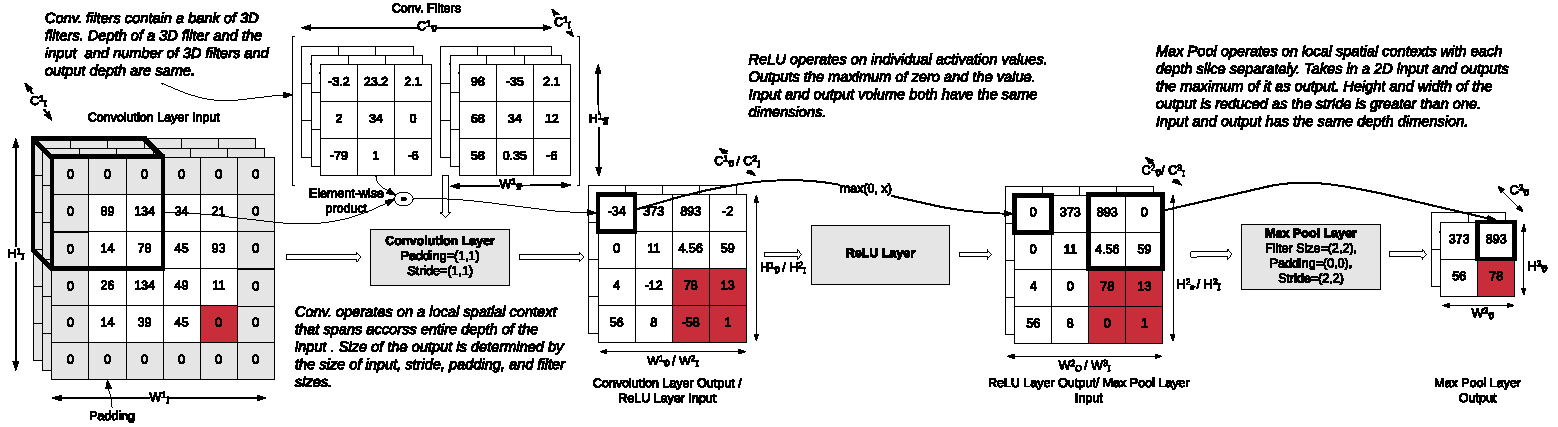
\includegraphics[width=\textwidth]{images/cnn_simplified}
\caption{Simplified representation of selected layers of a Deep CNN. The values marked in red show how a small spatial update in the first input would propagate through subsequent layers. (a) Convolution layer (for simplicity addition of bias is not shown in the Convolution transformation), (b) ReLU layer, and (c) Pool layer. Notation is explained in Table ~\ref{table:preliminaries_symbols}.}
\label{fig:cnn_simplified}
\end{figure*}

\begin{itemize}
    \item Transformations that operate at the granularity of a global context.
    \begin{itemize}
     \item E.g. Fully-Connected
    \end{itemize}
	\item Transformations that operate at the granularity of individual  spatial locations.
	\begin{itemize}
	 \item E.g. ReLU, Batch Normalization
	\end{itemize}
	\item Transformations that operate at the granularity of a local spatial context.
	\begin{itemize}
	 \item E.g. Convolution, Pooling
	\end{itemize}
\end{itemize}

\vspace{2mm}
\noindent \textbf{Transformations that operate at the granularity of a global context.} These transformations operate on a global context and does not take into account the spatial information.
Fully-Connected, which is the only global transformation layer in a CNN, takes in a 1-D tensor or a flattened 3-D tensor and performs a matrix-vector multiplication with a weight matrix and produces an output 1-D tensor.
Since it performs one bulk transformation, there is almost no substantial opportunity for exploiting redundancies with incremental computations.
The computational cost of a Full-Connected transformation is proportional to the product of the size of the input and output 1-D tensors.
Fully-Connected layers are used as the last or last few layers in a CNN and only accounts for a small fraction of the total computational cost.
Thus we ignore them henceforth.

\vspace{2mm}
\noindent \textbf{Transformations that operate at the granularity of individual  spatial locations.} These transformations essentially perform a $map(.)$ function on each individual element in the tensor (see Figure \ref{fig:cnn_simplified} (b)).
Hence, the output will have the same dimensions as input.
The computational cost incurred by these transformations is proportional to the volume of the input (or output).
However, with incremental spatially localized updates in the input, such as placing an occlusion patch, only the updated region needs to be recalculated.
Extending these transformations to become change aware is straightforward since they are element-wise operations.
The computational cost of the change aware incremental transformation is proportional to the volume of only the modified region.


\vspace{2mm}
\noindent \textbf{Transformations that operate at the granularity of a local spatial context.}
With incremental spatially localized updates in the input, transformations that operate at the granularity of a local spatial context also provide opportunities for exploiting redundancy and can be made change aware.
However, with local context transformations, such as Convolution and Pooling, this extension is non-trivial due to the overlapping nature of the spatial contexts.
% Convolution layers are the most important type of layer in the CNN architecture which also contributes to most of the computational cost.

Each Convolution layer can have $C_{\mathcal{O}:l}$ 3-D ``filter kernels'' organized into a 4-D array $\mathcal{K}_{conv:l}$, with each having a smaller spatial width $W_{\mathcal{K}:l}$ and height $H_{\mathcal{K}:l}$ compared to the width $W_{\mathcal{I}:l}$ and height $H_{\mathcal{I}:l}$ of the input tensor $\mathcal{I}_{:l}$, but has the same depth $C_{\mathcal{I}:l}$.
During inference, $c^{th}$ filter kernel is ``strided'' along the width and height dimensions of the input and a 2-D ``activation map'' $A_{:c}=(a_{y,x:c})\in \mathcal{\rm I\!R}^{H_{\mathcal{O}:l} \times~ W_{\mathcal{O}:l}}$ is produced by calculating element-wise products between the kernel and the input and adding a bias value as per Equation (\ref{eqn:elementwise_product}).
The computational cost of each of these individual element-wise products is proportional to the volume of the filter kernel.
Finally, these 2-D activation maps are stacked together along the depth dimension to produce an output tensor $\mathcal{O}_{:l} \in \mathcal{\rm I\!R}^{C_{\mathcal{O}:l} \times H_{\mathcal{O}:l} \times W_{\mathcal{O}:l}}$ as per Equation (\ref{eqn:conv_operator}).
A simplified representation of Convolution transformation is shown in Figure \ref{fig:cnn_simplified} (a).


\begin{align}
\label{eqn:elementwise_product}
\begin{split}
a_{y,x:c} =& \sum_{k=0}^{C_{\mathcal{I}:l} } \sum_{j=0}^{H_{\mathcal{K}:l}-1} \sum_{i=0}^{W_{\mathcal{K}:l}-1} \mathcal{K}_{conv:l}[c, k, j, i] \\
& \quad \times \mathcal{I}_{:l}[k,y-\floor{\frac{H_{\mathcal{K}:l} }{2}}+j,x-\floor{\frac{W_{\mathcal{K}:l} }{2}}+i] \\
& \quad + \mathcal{B}_{conv:l}[c]
\end{split}
\end{align}

\begin{align}
\label{eqn:conv_operator}
\begin{split}
\mathcal{O}_{:l} = [A_{:0}, A_{:1}, ... , A_{(C_{\mathcal{O}:l}-1)}]
\end{split}
\end{align}


% \eat{
% \begin{align}
% \begin{split}
% \text{Input Volume}:&~ \mathcal{I} \in \mathcal{\rm I\!R}^{C_{\mathcal{I}} \times H_{\mathcal{I}} \times W_{\mathcal{I}}}\\
% \text{Convolution Filters}:&~ \mathcal{K}_{conv} \in \mathcal{\rm I\!R}^{C_{\mathcal{O}} \times C_{\mathcal{I}} \times H_{\mathcal{K}} \times W_{\mathcal{K}}}\\
% \text{Convolution Bias Vector}:&~ \mathcal{B}_{conv} \in \mathcal{\rm I\!R}^{C_{\mathcal{O}}}\\
% \text{Output Volume}:&~ \mathcal{O} \in \mathcal{\rm I\!R}^{C_{\mathcal{O}} \times H_{\mathcal{O}} \times W_{\mathcal{O}}}
% \end{split}
% \end{align}

% \begin{equation}
% \label{eqn:conv_operator}
% \begin{split}
% \mathcal{O}[c,y,x] &= \sum_{k=0}^{C_{\mathcal{I}}} \sum_{j=0}^{H_\mathcal{K}-1} \sum_{i=0}^{W_\mathcal{K}-1} \mathcal{K}_{conv}[c, k, j, i] \\ & \quad \quad \quad \times \mathcal{I}[k,y-\floor{\frac{H_\mathcal{K}}{2}}+j,x-\floor{\frac{W_\mathcal{K}}{2}}+i] + \mathcal{B}[c]
% \end{split}
% \end{equation}
% }

Pooling can also be thought of as a Convolution operation with a fixed (i.e., not learned) 2-D filter kernel $\mathcal{K}_{pool:l}$.
But unlike Convolution, Pooling operates independently on each depth slice of the input tensor.
% The two main variations of pooling layers are max pooling (takes the maximum value from the local spatial context) and average (takes the average value from the local spatial context) pooling.
A Pooling layer takes a 3-D activation tensor $\mathcal{O}_{l}$ having a depth of $C_{\mathcal{I}:l}$, width of $W_{\mathcal{I}:l}$, and height of $H_{\mathcal{I}:l}$ as input and produces another 3-D activation tensor $\mathcal{O}_{:l}$ with the same depth of $C_{\mathcal{O}:l}=C_{\mathcal{I}:l}$, width of $W_{\mathcal{O}:l}$, and height of $H_{\mathcal{O}:l}$ as the output.
Pooling kernel is generally strided with more than one pixel at a time and hence $W_{\mathcal{O}:l}$ and $H_{\mathcal{O}:l}$ are generally smaller than $W_{\mathcal{I}:l}$ and $H_{\mathcal{I}:l}$.
A simplified representation of Pooling transformation is shown in Figure \ref{fig:cnn_simplified} (c).
% Similar to Convolution, Pooling operation can be formally defined as follows:

% \begin{align}
% \text{Pool Filters}:&~ \mathcal{K}_{pool} \in \mathcal{\rm I\!R}^{H_{\mathcal{K}} \times W_{\mathcal{K}}}
% \end{align}

% \begin{equation}
% \label{eqn:pool_operator}
% \begin{split}
% \mathcal{O}[c,y,x] &= \sum_{j=0}^{H_\mathcal{K}-1} \sum_{i=0}^{W_\mathcal{K}-1} \mathcal{K}_{pool}[j, i] \\ & \quad \quad \quad \times \mathcal{I}[c,y-\floor{\frac{H_\mathcal{K}}{2}}+j,x-\floor{\frac{W_\mathcal{K}}{2}}+i]
% \end{split}
% \end{equation}

It can be seen that Convolution and Pooling transformations can be cast into a form of applying a filter along the spatial dimensions of the 3-D input tensor.
However, how each transformation operates along the depth dimension is different.
For our purpose, since we are only interested in finding the spatial propagation of the patches in the input through the consecutive layers, both of these transformations can be treated similarly.

\vspace{2mm}
\noindent \textbf{Relationship between Input and Output Dimensions.}
The output tensor's dimensions $W_{\mathcal{O}:l}$ and $H_{\mathcal{O}:l}$ are determined by the dimensions of the input tensor $W_{\mathcal{I}:l}$ and $H_{\mathcal{I}:l}$, dimensions of the filter kernel $W_{\mathcal{K}:l}$ and $H_{\mathcal{K}:l}$ and two other parameters: \textbf{stride} $S_{:l}$ and \textbf{padding} $P_{:l}$.
Stride is the number of pixel values used to move the filter kernel at a time when producing a 2-D activation map.
It is possible to have two different values, with one for the width dimension $S_{x:l}$ and one for the height dimension $S_{y:l}$.
Generally $S_{x:l} \leq W_{\mathcal{K}:l}$ and $S_{y:l} \leq H_{\mathcal{K}:l}$.
In Figure \ref{fig:cnn_simplified}, Convolution transformation uses a stride value of 1 and Pool transformation uses a stride value of 2 for both dimensions.
Sometimes, in order to control the dimensions of the output tensor to be same as the input tensor, one needs to pad the input tensor with zeros around the spatial border.
Padding $P_{:l}$ captures the number of zeros that needs to be added.
Similar to the stride $S_{:l}$, it is possible to have two separate values for padding, with one for the width dimension $P_{x:l}$ and one for the height dimension $P_{y:l}$.
In Figure \ref{fig:cnn_simplified}, Convolution transformation pads the input with one line of zeros on both dimensions.
With these parameters defined, the width (similarly height) of the output tensor can be defined as follows:

\begin{align}
\begin{split}
W_{\mathcal{O}:l} = (W_{\mathcal{I}:l} - W_{\mathcal{K}:l} + 1 + 2\times P_{x:l})/S_{x:l} \\
% ^lH_{\mathcal{O}} = (^lH_{\mathcal{I}} - ^lH_\mathcal{K} + 1 + 2\times ^lP_y)/^lS_y
\end{split}
\end{align}

\vspace{2mm}
\noindent \textbf{Computational Cost of Deep CNNs.}
Deep CNNs are highly compute-intensive.
Of all the types of layers, Convolution layers almost always contribute to $90\%$ (or more) of the computation.
Hence, we can roughly estimate the computational cost of a Deep CNN by counting the number of fused multiply-add (FMA) floating point operations (FLOPs) required by Convolution layers for a single forward pass for inference.
% and ignore the computational cost of other layers (e.g. Pooling, Fully-Connected).

For example, applying a Convolution filter having the dimensions of ($C_{\mathcal{I}:l}$, $H_{\mathcal{K}:l}$, $W_{\mathcal{K}:l}$) to compute a single value in the output tensor will require $C_{\mathcal{I}:l} \times H_{\mathcal{K}:l} \times W_{\mathcal{K}:l}$ FLOPs, each corresponding to a single element-wise multiplication.
Thus, the total amount of computations $Q_{:l}$ required by that layer in order to produce an output tensor $\mathcal{O}_{:l}$ with dimensions $C_{\mathcal{O}:l} \times H_{\mathcal{O}:l} \times lW_{\mathcal{O}:l}$, and the total amount of computations $Q$ required to process the entire set of convolution layers $L$ in the CNN can be calculated as per Equation (\ref{eqn:full_local}) and (\ref{eqn:full_all}).

\begin{align}
\label{eqn:full_local}
Q_{:l} =&~ (C_{\mathcal{I}:l} \times H_{\mathcal{K}:l} \times W_{\mathcal{K}:l}) \times (C_{\mathcal{O}:l} \times H_{\mathcal{O}:l} \times W_{\mathcal{O}:l})\\
\label{eqn:full_all}
Q =&~ \sum_{l \in L}Q_{:l}
\end{align}


\eat{
\subsection{Estimating the Quality of Generated Approximate Heat Maps}

When applying approximate inference optimizations \system~ sacrifices the the accuracy/quality of the generated heat map in favor of faster execution.
To measure this drop of accuracy we use Structural Similarity (SSIM) Index~\cite{wang2004image} which is one of the widely used approaches to measure the \textit{human perceived difference} between two similar images.
When applying SSIM index we treat the original heat map as the reference image with no distortions and the perceived image similarity of the \system~generated heat map is calculated with reference to it.
The generated SSIM index is a value between $-1$ and $1$, where $1$ corresponds to perfect similarity.
% It is important to note that, even though SSIM index value of 1 corresponds to perfect similarity, other values doesn't necessarily imply same level of perceived quality across different image pairs.
% However, if the original images are closely similar, such as in chest X-ray images, it can be assumed that this condition will hold.
Typically SSIM index values in the range of $0.90-0.95$ are used in practical applications such as image compression and video encoding as at the human perception level they produce indistinguishable distortions.
For more details on SSIM Index method, we refer the reader to the original SSIM Index paper~\cite{wang2004image}.
}



%!TEX root = <main.tex>
\section{Experimental Evaluation}
We have integrated all of our optimization techniques from Sections 3 and 4 with the popular deep learning tool PyTorch to create a prototype tool we call \system.
We now evaluate the speedups yielded by \system~ for occlusion-based explanations for several deep CNNs on real-world image datasets.
We then drill into the contributions of each of our optimization techniques.

\vspace{2mm}
\noindent \textbf{Datasets.}
We use three diverse real-world image datasets: \textit{OCT}, \textit{Chest X-Ray}, and a sample from \textit{ImageNet}. \textit{OCT} has about 84,000 optical coherence tomography retinal images with four classes: CNV, DME, DRUSEN, and NORMAL. CNV (choroidal neovascularization), DME (diabetic macular edema), and DRUSEN are three varieties of diabetic retinopathy. NORMAL corresponds to healthy retinal images. \textit{Chest X-Ray} has about 6,000 X-ray images with three classes: VIRAL, BACTERIAL, and NORMAL. VIRAL and BACTERIAL are two varieties of pneumonia. NORMAL corresponds to healthy people. Both \textit{OCT} and \textit{Chest X-Ray} are from a recent scientific study that applied deep CNNs to radiology images to detect the respective diseases~\cite{kermany2018identifying}. \textit{ImageNet} is a benchmark dataset in computer vision~\cite{deng2009imagenet}; our sample has 1,000 images with 200 classes.

\vspace{2mm}
\noindent \textbf{Workloads.}
We use 3 popular ImageNet-trained deep CNNs: VGG16~\cite{vggnet}, ResNet18~\cite{resnet}, and Inception3~\cite{inception}, obtained from~\cite{torchvisionmodels}. They complement each other in terms of model size, architecture complexity, computational cost, and our predicted theoretical speedups for OBE with incremental inference (Figure 3 in Section 3). For \textit{OCT} and \textit{Chest X-Ray}, the 3 CNNs were fine-tuned by retraining their final Fully-Connected layers as per standard practice. The details of fine-tuning are not relevant for the rest of our discussion; so, we present further details in the Appendix. The OBE heat maps are plotted using Python Matplotlib's \texttt{imshow} method using the \texttt{jet\_r} color scheme; we set the maximum threshold to \texttt{min}$(1, 1.25 p)$ and minimum to $0.75 p$, where $p$ is predicted class probability on a given image. All images are resized to the input size required by the CNNs ($224\times224$ for VGG16 and ResNet18; $299\times299$ for Inception3); no additional pre-processing was done. The GPU-based experiments used a batch size of $128$; for CPUs, the batch size was $16$. All CPU-based experiments were executed with a thread parallelism of $8$. All of our datasets, experimental scripts, and the \system~ codebase will be made publicly available on our project webpage.

\vspace{2mm}
\noindent \textbf{Experimental Setup.}
We use a machine with 32 GB RAM, Intel i7-6700 3.40GHz CPU, and NVIDIA Titan X (Pascal) GPU with 12 GB memory. %1 TB Seagate ST1000DM010-2EP1
The machine runs Ubuntu 16.04 with PyTorch version 0.4.0, CUDA version 9.0, and cuDNN version 7.1.2.
All reported runtimes are the average of 3 runs, with 95\% confidence intervals shown.

\subsection{End-to- End Runtimes}

\begin{figure*}[t]
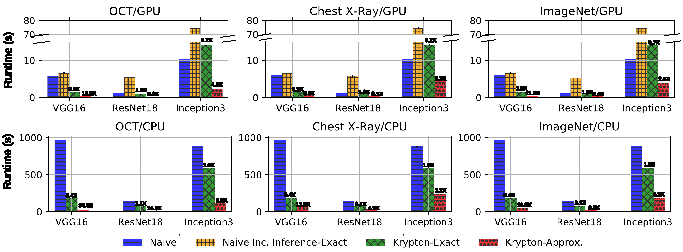
\includegraphics[width=\textwidth]{images/5_1_all_edited_b}
\vspace{-6mm}
\caption{End-to-end runtimes of \system~ and baselines on all 3 datasets, 3 CNNs, and both GPU and CPU.}
\label{fig:5_1_all_edited}
\end{figure*}

We focus on the most common OBE scenario of producing the whole heat map, i.e., $G$ is automatically created (``non-interactive'' mode). We use an occlusion patch of size 16 and stride 4. We compare two variants of \system: \system-Exact uses only incremental inference (Section 3), while \system-Approximate uses our approximate inference optimizations too (Section 4). The main baseline is \textit{Naive}, the current dominant practice of performing full inference for OBE with just naive batching of images. We have another baseline for the GPU environment: \textit{Naive Inc.~Inference-Exact}, which is a direct implementation of Algorithm~\ref{alg:incinference} in PyTorch/Python without using our GPU-optimized CUDA kernel, which \system~ uses (Section 3.4). Note that \textit{Naive Inc.~Inference-Exact} is not applicable to the CPU environment.

We set the user-given tuning parameters for adaptive drill-down based on the semantics of each dataset's prediction task (Section 4.3). For \textit{OCT}, since the region of interest is likely to be small, we set $r_{drill-down}=0.1$ and $\mathit{target} = 5$. For \textit{Chest X-Ray}, the region of interest can be large; so, we set $r_{drill-down} = 0.4$ and $\mathit{target} = 2$. For \textit{ImageNet}, which falls in between, we use the \system~ default values of $r_{drill-down}=0.25$  and $\mathit{target} = 3$. For all experiments $\tau$ is auto-tuned with a target SSIM of $0.9$ (Section 4.3). Figure~\ref{fig:5_1_all_edited} presents the results. Visual examples of images and the heat maps produced are presented in the Appendix.

Overall, we see \system~ offers significant speedups across the board on both GPU and CPU. The highest speedups are reported by \system-Approximate on \textit{OCT} with VGG16: $16$X on GPU and $34.5$X on CPU. The highest speedups of  \system-Exact are also on VGG16: $3.9$X on GPU and $5.4$X on CPU. The speedups of \system-Exact are identical across datasets for a given CNN, since it does not depend on the image semantics, unlike \system-Approximate due to its data-dependent parameters. \system-Approximate reports the highest speedups on \textit{OCT} because our auto-tuning yielded the lowest $\tau$, highest target speedup, and lowest $r_{drill-down}$ on that dataset. 

The speedups are lower with ResNet18 and Inception3 than VGG16 due to their architectural properties (kernel filter dimensions, stride, etc.) that make the projective field grow faster. Moreover, Inception3 has a complex DAG architecture with more branches and depth-wise concatenation, which limits GPU throughput for incremental inference. In fact, \system-Exact on GPU shows a minor slow-down ($0.7$X) with Inception3. But \system-Approximate still offers speedups on GPU with Inception3 (up to $4.5$X). We also see that ResNet18 and VGG16 almost near their theoretical speedups (Figure~\ref{fig:redundancy_ratio}) but Inception3 does not. Note that the theoretical speedup definition only counts FLOPs and does not account for memory stalls.

Finally, the speedups of \system~ are higher on CPU than GPU. This is because CPU does not suffer much due to memory stalls during incremental inference. But the \textit{absolute} runtimes are almost an order of magnitude higher on CPUs than GPUs, which is to be expected. Overall, \system~ improves the efficiency of OBE significantly for multiple datasets and deep CNNs. We ran an additional experiment on the ``interactive'' mode by reducing $|G|$. The speedups go down as $|G|$ goes down, which is expected because the benefits of amortization are reduced. Due to space constraints, these additional results are presented in the Appendix.


\subsection{Lesion Study}
We now analyze the contributions of our 3 optimizations individually. We compare the speedups of \system~ over \textit{Naive} (batched inference) on both CPU and GPU, termed  Empirical-CPU and Empirical-GPU respectively, against the theoretical speedups (explained in Sections 3 and 4).
%% Does not matter. It can be any arbitary input image. We are not tuning.
% All experiments use an image from the \textit{OCT} dataset (\red{TODO: Check}) and produce the full heat maps.

\begin{figure}[t]
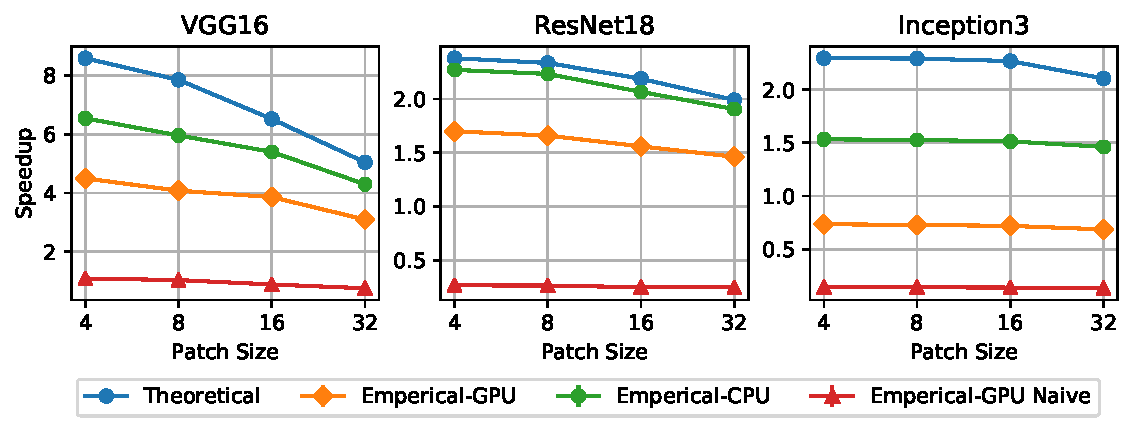
\includegraphics[width=\columnwidth]{images/5_2_1_edited}
\vspace{-8mm}
\caption{Speedups with only the incremental inference optimization (occlusion patch stride $S=4$).}
\label{fig:5_2_1_edited}
\end{figure}

\vspace{2mm}
\noindent \textbf{Only Incremental Inference.} 
We vary the patch size and set the stride to $4$. Figure~\ref{fig:5_2_1_edited} shows the results. As expected, the speedups go down as the patch size increases. Empirical-GPU Naive yields no speedups because it does not use our GPU-optimized kernel, while Empirical-GPU does. But Empirical-CPU is closer to theoretical speedup and almost matches it on ResNet18. Thus, there is still some room for improvement to improve the efficiency of incremental inference in both environments.


\begin{figure}[t]
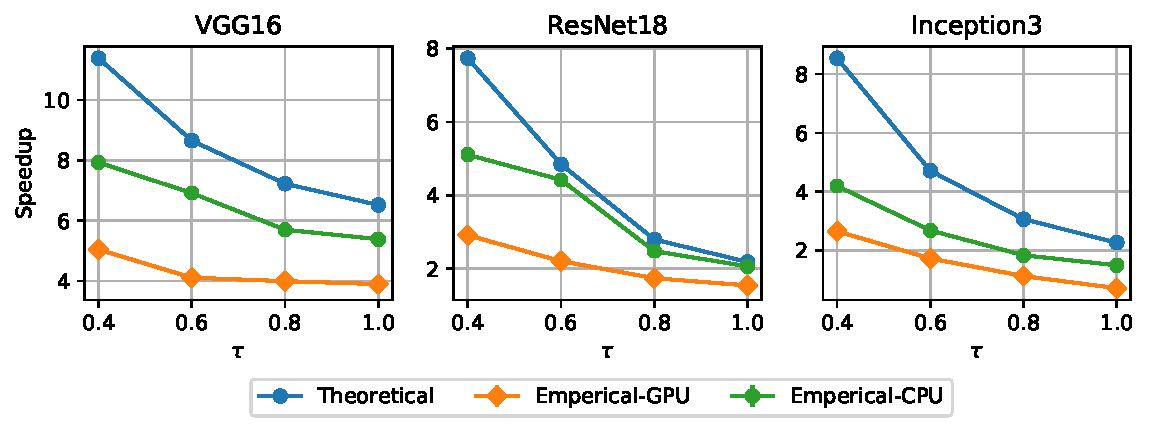
\includegraphics[width=\columnwidth]{images/5_2_2_edited}
\vspace{-8mm}
\caption{Speedups with incremental inference combined with only projective field thresholding (occlusion patch size$=16$, stride $S=4$).}
\label{fig:5_2_2_edited}
\end{figure}

\vspace{2mm}
\noindent \textbf{Projective Field Thresholding.} We vary $\tau$ from $1.0$ (no approximation) to $0.4$. Adaptive drill-down is disabled but note that this optimization builds on top of our incremental inference. The occlusion patch size is $16$ and stride is $4$. Figure~\ref{fig:5_2_2_edited} shows the results. The speedups go up steadily as $\tau$ drops for all 3 CNNs. Once again, Empirical-CPU nears the theoretical speedups on ResNet18, but the gap between Empirical-GPU and Empirical-CPU remains due to the disproportionate impact of memory stalls on GPU. Overall, this approximation offers some speedups in both environments, but has a higher impact on CPU than GPU.

\begin{figure}[t]
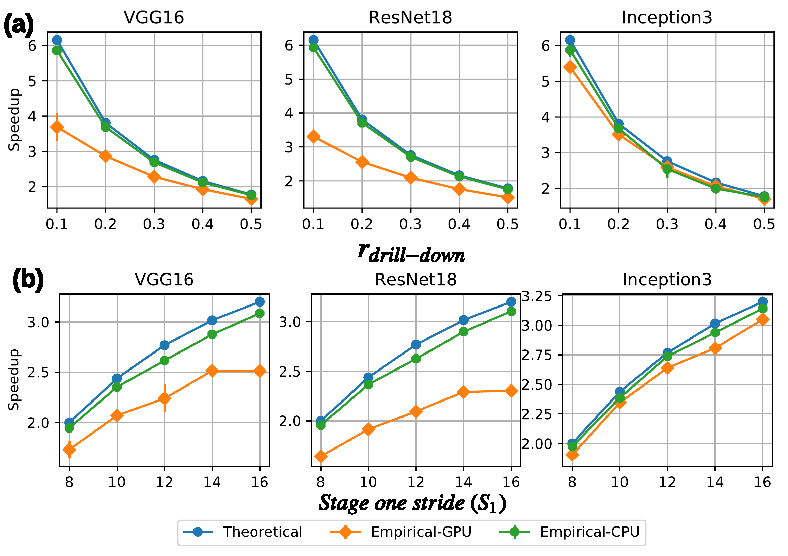
\includegraphics[width=\columnwidth]{images/5_2_3_edited}
\vspace{-8mm}
\caption{Speedups with incremental inference combined with adaptive drill-down. For (a), we set $S_1=16$. For (b), we set $r_{drill\_down}=0.25$).}
\label{fig:5_2_3_edited}
\end{figure}

\vspace{2mm}
\noindent \textbf{Adaptive Drill-Down.} Finally we study the effects of adaptive drill-down (again, on top of incremental inference) and disable projective field thresholding. The occlusion patch size is $16$. Stage two stride is $S_2 = 4$. First, we vary $r_{drill-down}$, while fixing stage one stride ($S_1 = 16$). Figure~\ref{fig:5_2_3_edited}(a) shows the results. Next, we vary $S_1$, while fixing $r_{drill-down} = 0.25$. Figure~\ref{fig:5_2_3_edited}(b) shows the results. As expected, the speedups go up as $r_{drill-down}$ goes down or $S_1$ goes up, since fewer re-inference queries arise in both cases. Empirical-CPU almost matches the theoretical speedups across the board; in fact, even Empirical-GPU almost matches theoretical speedups on Inception3. Empirical-GPU flattens out at high $S_1$, since the number of re-inference queries drops, thus resulting in diminishing returns for the benefits of batched execution on GPU. Overall, this optimization has a major impact on speeding up OBE for all CNNs in both environments.

\vspace{2mm}
\noindent \textbf{Summary of Experiments.} Overall, our empirical evaluation shows that \system~ is able to substantially accelerate the OBE workload for explaining CNN predictions, up to $16$X speedups on GPU and $34.5$X speedups on CPU. The speedups of all 3 of our optimizations depend on the CNN's architectural properties. The speedups of our approximate inference optimizations also depend on the dataset due to their tunable parameters, which \system ~can tune automatically. Finally, the speedups of \system ~are higher on CPU than GPU but the absolute runtimes are much lower on GPU. Overall, all of our optimizations in \system ~help reduce waiting times for users and can save resource costs, since they only using existing compute resources without forcing users to pay for more resources (say, renting more GPUs in the cloud).

\bibliographystyle{abbrv}
\bibliography{main}
\end{document}